\documentclass[smaller,dvipsnames]{beamer}

\usetheme[numbering=fraction,%
          block=fill,%
          sectionpage=progressbar,%
          subsectionpage=progressbar,%
]{metropolis} % Use metropolis theme
\setbeamercovered{invisible}

\usepackage[utf8]{inputenc}
\usepackage[T1]{fontenc}
%\usepackage[dvipsnames]{xcolor}
\usepackage{xspace}
\usepackage{booktabs}
\usepackage{amssymb}
\usepackage{tikz}
\usetikzlibrary{arrows} % required in the preamble
\usepackage{smartdiagram}
\usesmartdiagramlibrary{additions} % required in the preamble
\usepackage{listings}

\newcommand{\myplus}{\textcolor{ForestGreen}{\textbf{+}}}
\newcommand{\myminus}{\textcolor{red}{\textbf{$-$}}}
\newcommand{\ah}{Angry-HEX\xspace}
\newcommand{\ab}{Angry Birds\xspace}
\newcommand{\abc}{Angry Birds AI Competition\xspace}
\newcommand{\al}{Alpha\xspace}

\title{Complex Predicates vs.\ Complex Objects}
\subtitle{A Case Study on ASP for Implementing Artificial Agents}
\author{Filippo De Bortoli \and Lorenz Leutgeb \and Cosimo Persia}
\institute{European Master's Program in Computational Logic, TU Dresden}
\date{February 16th, 2018}

\begin{document}

\maketitle

\begin{frame}{Outline}
    \tableofcontents
\end{frame}

\section{Introduction}

\subsection{Angry Birds}

\begin{frame}{The Game}
	\begin{figure}
  		
\includegraphics[width=300pt]{./img/angry-birds.jpg}
	\end{figure}
	\begin{itemize}
		\item<1-> Eliminate all pigs
		\item<2-> Reach high score
	\end{itemize}
\end{frame}

\begin{frame}{Challenges for AI}
	 \begin{columns}
		 \begin{column}{0.5\textwidth}
			\begin{itemize}
				\item<1->[] Physics
				{\par\centering\includegraphics<1>[width=4.5cm]{./img/birds-square}\par}
				\item<2->[] Planning
				{\par\centering\includegraphics<2>[width=4.5cm]{./img/planning.png}\par}
			\end{itemize}
		 \end{column}
		 \begin{column}{0.5\textwidth}
			\begin{itemize}
			\item<3->[] Computer Vision
    		{\par\centering\includegraphics<3>[width=4.5cm]{./img/object-detection}\par}
    		\item<4->[] Knowledge Representation
  		\end{itemize}
		 \end{column}
	 \end{columns}
\end{frame}

\subsection{Motivation}

\begin{frame}{Motivation}
	\begin{itemize}[<+->]
		\item Find an existing agent based on logic programming (ASP). \newline \(\rightarrow\) Angry-HEX
		\item Understand how it works.
		\item Adapt it to the Alpha system to find out how it can be improved from an application programmers perspective.
		\item Structure and formalize the learnings.
		\item Improve the agent overall!
	\end{itemize}
\end{frame}

\section{Preliminaries}

\subsection{Answer Set Programming}

\begin{frame}{Declarative Programming}
 	\begin{center}
 	\begin{itemize}
	\item<1->[] \begin{center} {\large{ALGORITHM = LOGIC + CONTROL}} \end{center}
		\begin{align*}
			&append ([\:], X, X). \\
			&append ([X|Y], Z, [X|T ]) \leftarrow append (Y, Z, T ). \\
			&reverse([ ], [ ]).\\
			&reverse([X|Y ], Z) \leftarrow append (U, [X], Z), reverse(Y, U ).
		\end{align*}
  \item<2>[] Order of clauses and subgoals does not matter.
  		\begin{align*}
			reverse([X|Y], Z) \leftarrow reverse(Y, U ), append (U, [X], Z).
		\end{align*}
	\end{itemize}	
	\end{center}
\end{frame}

\begin{frame}{Stable Model Semantics}
    \begin{center}
    	\begin{align*}
			&pig((88,34)). \\
			&easy\_target(X) \leftarrow pig(X), not\: difficult\_target(X). \\ 
			&difficult\_target(X) \leftarrow pig(X), not\: easy\_target(X). 
		\end{align*}
    \end{center}
    \begin{itemize}
    	\item<2->[] Models that reflect natural intuition.
    	\item<3->[]
    		\begin{align*}
				&\only<4>{\alert}{ M_1= \{pig((88,34)), easy\_target((88,34))\}  } \\
				&\only<4>{\alert}{ M_2= \{pig((88,34)), difficult\_target((88,34))\}  }\\
				&M_3= \{pig((88,34)), easy\_target((88,34)), difficult\_target((88,34))\}
    		\end{align*}
    \end{itemize}
\end{frame}

\begin{frame}{Stable Model Semantics}
	\begin{center} {\large{Gelfond Lifschitz Reduct}} \end{center}
	Given a program \(P\) and an interpretation \(M\), its \emph{reduct} \(P^M\) is the program reduced obtained by 
	\begin{enumerate}
		\item removing rules with \(\text{not } a\) in the body for each \(a \in M\)
		\item removing literals \(\text{not } a\) from all other rules.
	\end{enumerate}	  
	We say that \(M\) is a stable model if the least model of \(P^M\) coincides with \(M\).
\end{frame}

\subsection{HEX-Programs}

\begin{frame}{Higher Order Atoms}
	Higher order atoms are atoms that have predicate symbols as arguments.
	\begin{itemize}[<+->]
		\item[] \(p(a),p(b),p(c)\) \quad \quad \quad \quad \quad ordinary, unary atoms
		\item[] \(h(\alert{p},I) \leftarrow \alert{p}(I).\) \quad \quad \quad \quad \quad higher order atom
		\item[] \alert{first order atom}
	\end{itemize}
\end{frame}

\begin{frame}{External Atoms}
    \begin{itemize}[<+->]
    	\item They allow bidirectional communication with external sources: \[ \&g[q_1,\dots,q_k](t_1,\dots,t_l) \]
    	\item For example, use an arbitrary computable function to access an RDF file from the web: \[ \&rdf[url](X,Y,Z) \]
    	\item Returned result can be used as usual:
    		\begin{align*}
				analyze(X,Y,Z) \leftarrow \&rdf[url](X,Y,Z)
    		\end{align*}
    	\item Can be used for numeric computation (physics, e.g.~trajectories).
    \end{itemize}
\end{frame}

\begin{frame}{HEX-programs}
    \begin{itemize}[<+->]
    	\item Generalization of disjunctive extended logic programs under the answer set semantics.
    	\item External atoms \[ \&g[q_1,\dots,q_k](t_1,\dots,t_l) \]
    	\item Rules \[ a_1 \lor \dots \lor a_k \leftarrow b_1, \dots , b_n, \text{not } b_{n+1}, \dots, \text{not } b_m \quad (k,m,n \geq 0)\] where \(b_1, \dots, b_m\) may be (higher-order) external atoms and \(a_1, \ldots a_k\) may be higher-order but not external atoms. 
    \end{itemize}
\end{frame}

\section{\ah}

\begin{frame}{\ah Architecture}
	\begin{center}
		\begin{figure}
			\begin{tikzpicture}
				\node[anchor=south west,inner sep=0] at (0,0) {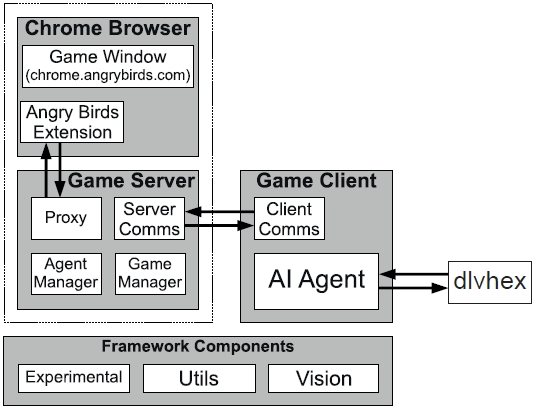
\includegraphics[scale=0.6]{./img/angryhex-agent}};
				\begin{uncoverenv}<2->
					\draw[ForestGreen,line width=3pt] (4.3,0.3) rectangle (6.0,0.7);
				\end{uncoverenv}
				\begin{uncoverenv}<3->
					\node[anchor=south, blue] (plan) at (5.5,5.4) {\Large Planning};
					\draw[blue,ultra thick,rounded corners] (5.0,1.65) rectangle (5.95,2.4);
					\draw [-stealth, blue,ultra thick,rounded corners] (plan) -- (5.45,2.5);
					\node[anchor=west, blue] (tactic) at (7.1, 6.0) {Tactic};
					\node[anchor=west, blue] (strategy) at (7.1, 5.3) {Strategy};
					\draw [-stealth, blue,ultra thick,rounded corners] (strategy) -- (6.5,5.6);
					\draw [-stealth, blue,ultra thick,rounded corners] (tactic) -- (6.5,5.8);
				\end{uncoverenv}
				\begin{uncoverenv}<4->
					\draw[alerted text.fg,ultra thick,rounded corners] (7.1,1.6) -- (8.5,2.4);
					\draw[alerted text.fg,ultra thick,rounded corners] (7.1,2.4) -- (8.5,1.6);
					\node[text=alerted text.fg] at (7.8,2.8) {\Large Alpha};	
				\end{uncoverenv}
			\end{tikzpicture}
			\caption{Agent architecture, from \emph{Angry-HEX: An Artificial Player for Angry Birds Based on Declarative
			Knowledge Bases}, Calimeri et al., 2016}
		\end{figure}
	\end{center}
\end{frame}

\begin{frame}{Interaction with HEX-programs: Tactic}
	\begin{center}
		\smartdiagramset{
        circular final arrow disabled=false,
        circular distance=2.25cm,
        arrow tip=to,
        arrow line width=2pt,
        additions={
            additional item offset=0.65cm,
            additional arrow line width=2pt,
            additional arrow tip=to,
            additional arrow color=orange!60!yellow,
        }
    }
    \smartdiagramadd[circular diagram]{
    Answer Set,Game Action,Game Level,Facts $\mathcal{S}$,$\mathcal{P}_{AI} \cup \mathcal{S}$
    }{
    left of module3/%
	}
	% game action -> shoot the target
    \smartdiagramconnect{to-}{module3/additional-module1}
\end{center}
\(\mathcal{P}_{AI}\) denotes the collection of HEX-programs used by \ah
\end{frame}

\begin{frame}{Interaction with HEX-programs: Strategy}
	The agent plays levels, according to this \alert{strategy}:
	\begin{enumerate}
		\item Play each level once
		\item Play those levels where \ah score differs the most from best overall score
		\item Play levels in which \ah played best and difference to 2nd best score is minimal
		\item To break ties, play random levels
	\end{enumerate}
\end{frame}

\begin{frame}{DLV-HEX vs.\ \al}
	\begin{center}
		\begin{tabular}{lcc}
			\toprule
			& \textbf{DLV-HEX} & \textbf{\al} \\
			\midrule
			\alert{Term Interpretation} & & \\
			~~~Constants & \checkmark & \checkmark \\
			~~~Natural Numbers & \checkmark & \checkmark \\
			~~~Quoted Strings & \checkmark & \checkmark \\
			~~~Java Objects & & \checkmark \\
			\midrule
			\alert{HEX-Programs} & & \\
			~~~Higher Order Atoms & \checkmark & \\
			~~~External Atoms & \checkmark & \checkmark \\
			\bottomrule
		\end{tabular}
	\end{center}
	How to \alert{convert} external and higher-order atoms to first-order external atoms, using Java objects as interpretation for terms?
\end{frame}

\section{From Complex Predicates to Complex Objects}

\begin{frame}{Encoding Sets using Complex Predicates}
	A set \(hills = \{ a, b, c \}\):
    \begin{align*}
    	hills(a).~~hills(b).~~hills(c). \\
    \end{align*}

	Quantify over \(hills\):
	\begin{align*}
		r(obstacles,hills). \\
		Z(X) \leftarrow r(Z,Y), Y(X).
	\end{align*}
\end{frame}

\begin{frame}{Encoding Sets using Complex Objects}
	\begin{itemize}[<+->]
	\item{\texttt{Set<T> hills = Set.of(a, b, c);}
    \begin{align*}
    	hills(o).
    \end{align*}

	where \(o\) is interpreted as the Java object \texttt{hills}.}


	\item{Quantify over \(hills\):
	\begin{align*}
		obstacles(X) \leftarrow hills(X).
	\end{align*}}
	
	\item{Deconstruct \(hills\):
	\begin{align*}
		firstHill(X) \leftarrow hills(H),\ \#head(H,X).
	\end{align*}}
	\end{itemize}
\end{frame}

\begin{frame}{Angry-HEX Codebase}
	\begin{itemize}[<+->]
		\item Implementations of external sources in a 2694 SLOCs mess of C++.
		\item Chaotic Java glue that interfaces with the \ab Challenge {framework} and DLV-HEX.
		\item Development spikes every year before the Angry Birds AI Competition.
		\item Objects relevant for reasoning are inserted into ASP programs as facts.
	\end{itemize}
\end{frame}

\begin{frame}[fragile]{Traces in \ah}
\begin{lstlisting}[language=C++,basicstyle=\ttfamily\small,keywordstyle=\alert]
for (ComfortInterpretation::iterator c = i.begin();
     c != i.end(); ++c) {
  if (c->getPredicate() == "objects") {
    Object o;
    o.id = c->getArgument(1).intval;
    if (c->getArgument(2).getUnquotedString() == "ice")
      o.type = ice;
    else if (c->getArgument(2).getUnquotedString()
             == "wood")
      o.type = wood;
    ...
  } else if (c->getPredicate() == "hills") {
    // handle polygon objects (hills)
    int id = c->getArgument(1).intval;
    int idx = c->getArgument(2).intval;
    int x = c->getArgument(3).intval;
    int y = c->getArgument(4).intval;
\end{lstlisting}
\end{frame}

\begin{frame}{Implementation of External Sources}
	Evaluation of the rule
	    $$ canPush(A,B) \leftarrow world(W), \textcolor{ForestGreen}{\&}\alert{canPush}\textcolor{Fuchsia}{[}\textcolor{blue}{W}\textcolor{Fuchsia}{]}\textcolor{Red}{(A,B)} \label{main:rule-3} $$
	    
	where \(W\) contains the state of the world to be reasoned about will invoke the Java method

    \texttt{\hspace{3mm}\textcolor{ForestGreen}{@Predicate}\\\hspace{3mm}Set<\textcolor{Red}{List<ConstantTerm>}\-> \alert{canPush}\textcolor{Fuchsia}{(}ASPWorld \textcolor{blue}{aspWorld}\textcolor{Fuchsia}{)}}
    
    Note that types are preserved: Throws if instance of \(W\) is not an \texttt{ASPWorld})!
\end{frame}

\begin{frame}{Pros and Cons of our Modifications}
	\begin{itemize}[<+->]
		\item[\myplus] Improved interoperability between glue code in Java and ASP system.
		\item[\myplus] Ordinary ASP programs are easier to read and understand than higher-order programs.
		\item[\myplus] Alpha uses lazy-grounding (maybe beneficial in the future).
		\item[\myminus] ASP system not as mature (no optimization, contributions welcome).
		\item[\myminus] Reinvention of DLV-Complex?
	\end{itemize}
\end{frame}

\begin{frame}
	\frametitle{Complexity}
	\begin{itemize}
		\item \(\mathcal{P}_{AI}\) is \alert{disjunction-free}
		\item We assume that \alert{external sources} have complexity in \(NP\) (no formal proofs at the moment)
		\item Thus, the \alert{complexity} of the reasoning process is \textsc{NExpTime}\textsuperscript{\textsc{NP}}
	\end{itemize}
	This theoretical result comes from \emph{A Uniform Integration of Higher-Order Reasoning and External Evaluations
	in Answer-Set Programming}, Eiter, Ianni, Schindlauer \& Tompits, 2005.
\end{frame}

\begin{frame}{Recap}
    \tableofcontents
\end{frame}

\begin{frame}[standout]
    Thank you!
\end{frame}

\end{document}